\documentclass[aspectratio=169, 10pt]{beamer}

% Theme & Styling (Clean Academic Look)
\usetheme{Madrid}
\usecolortheme{whale}
\setbeamertemplate{navigation symbols}{}
\setbeamertemplate{headline}{}

% Packages
\usepackage{amsmath, amssymb}
\usepackage{booktabs}
\usepackage{graphicx}
\usepackage{siunitx}

% Metadata
\title[1D Premixed Flame Simulation]{1D Premixed Methane-Air Combustion Simulation}
\subtitle{Numerical Analysis using Detailed Chemical Kinetics (Cantera \& GRI-Mech 3.0)}
\author{Mohit}
\institute[Dept. of Thermal Engg.]{Department of Mechanical / Thermal Engineering}
\date{\today}

\begin{document}

% -----------------------------------------------------------------------------
% Title Slide
% -----------------------------------------------------------------------------
\begin{frame}
  \titlepage
\end{frame}

% -----------------------------------------------------------------------------
% Slide 1: Problem Definition & Objectives
% -----------------------------------------------------------------------------
\begin{frame}{Problem Definition \& Objectives}
\begin{columns}[T]
  \begin{column}{0.55\textwidth}
    \textbf{Objective:}
    \begin{itemize}
      \item Model a stationary, 1D freely-propagating premixed laminar flame.
      \item Perform parametric sweep across equivalence ratio ($\phi = 0.70$ to $1.30$).
    \end{itemize}
    \vspace{0.8em}
    \textbf{Key Quantities Evaluated:}
    \begin{itemize}
      \item Laminar Flame Speed ($S_L$) as an eigenvalue.
      \item Maximum flame temperature ($T_{\max}$) and adiabatic equilibrium.
      \item Internal flame zones (Preheat layer vs.\ Reaction zone).
      \item Radical pool concentrations ($OH, H, O, HO_2$).
    \end{itemize}
  \end{column}

  \begin{column}{0.42\textwidth}
    \begin{block}{Flame Assumptions}
      \begin{itemize}
        \item Planar, 1D freely-propagating flame.
        \item Ambient inlet: $T_u = 300\text{ K}$, $P = 1\text{ atm}$.
        \item Dry atmospheric air: $O_2 : N_2 = 1 : 3.76$.
        \item Steady-state 1D eigenvalue formulation.
      \end{itemize}
    \end{block}
  \end{column}
\end{columns}
\end{frame}

% -----------------------------------------------------------------------------
% Slide 2: Governing Equations
% -----------------------------------------------------------------------------
\begin{frame}{Governing Conservation Equations}
The one-dimensional steady flame structure satisfies the coupled boundary-value system:

\begin{block}{1. Mass Conservation (Continuity)}
$$\frac{d(\rho u)}{dx} = 0 \quad \implies \quad \dot{m} = \rho u = \text{constant}$$
\end{block}

\begin{block}{2. Species Conservation (for each species $k = 1, \dots, K$)}
$$\dot{m} \frac{d Y_k}{dx} = -\frac{d j_k}{dx} + \dot{\omega}_k W_k$$
\end{block}

\begin{block}{3. Energy Conservation}
$$\dot{m} c_p \frac{dT}{dx} = \frac{d}{dx}\left(\lambda \frac{dT}{dx}\right) - \sum_{k=1}^K j_k c_{p,k} \frac{dT}{dx} - \sum_{k=1}^K h_k \dot{\omega}_k W_k$$
\end{block}
\end{frame}

% -----------------------------------------------------------------------------
% Slide 3: Solver & Mechanism Setup
% -----------------------------------------------------------------------------
\begin{frame}{Chemical Kinetics \& Numerical Methods}
\begin{columns}[T]
  \begin{column}{0.5\textwidth}
    \textbf{Kinetic Mechanism: GRI-Mech 3.0}
    \begin{itemize}
      \item 53 chemical species, 325 elementary reactions.
      \item Industry benchmark for methane combustion.
      \item NASA polynomials for thermodynamic properties ($c_p, h, s$).
      \item Mixture-averaged transport model ($\lambda, \mu, D_{km}$).
    \end{itemize}
  \end{column}

  \begin{column}{0.5\textwidth}
    \textbf{Cantera Numerical Strategy}
    \begin{itemize}
      \item \textbf{Eigenvalue Problem:} Damped Newton-Raphson iteration solves for $S_L = u(0)$.
      \item \textbf{Adaptive Mesh Refinement:}
        \begin{itemize}
          \item Initial grid: 16 points.
          \item Refinement criteria: \texttt{slope=0.05}, \texttt{curve=0.08}.
          \item Final converged grid: 196--236 non-uniform points clustered inside the reaction zone.
        \end{itemize}
    \end{itemize}
  \end{column}
\end{columns}
\end{frame}

% -----------------------------------------------------------------------------
% Slide 4: Results — Flame Speed & Max Temperature vs Phi
% -----------------------------------------------------------------------------
\begin{frame}{Results: Flame Speed \& Temperature vs Mixture Strength}
\begin{columns}[c]
  \begin{column}{0.52\textwidth}
    \centering
    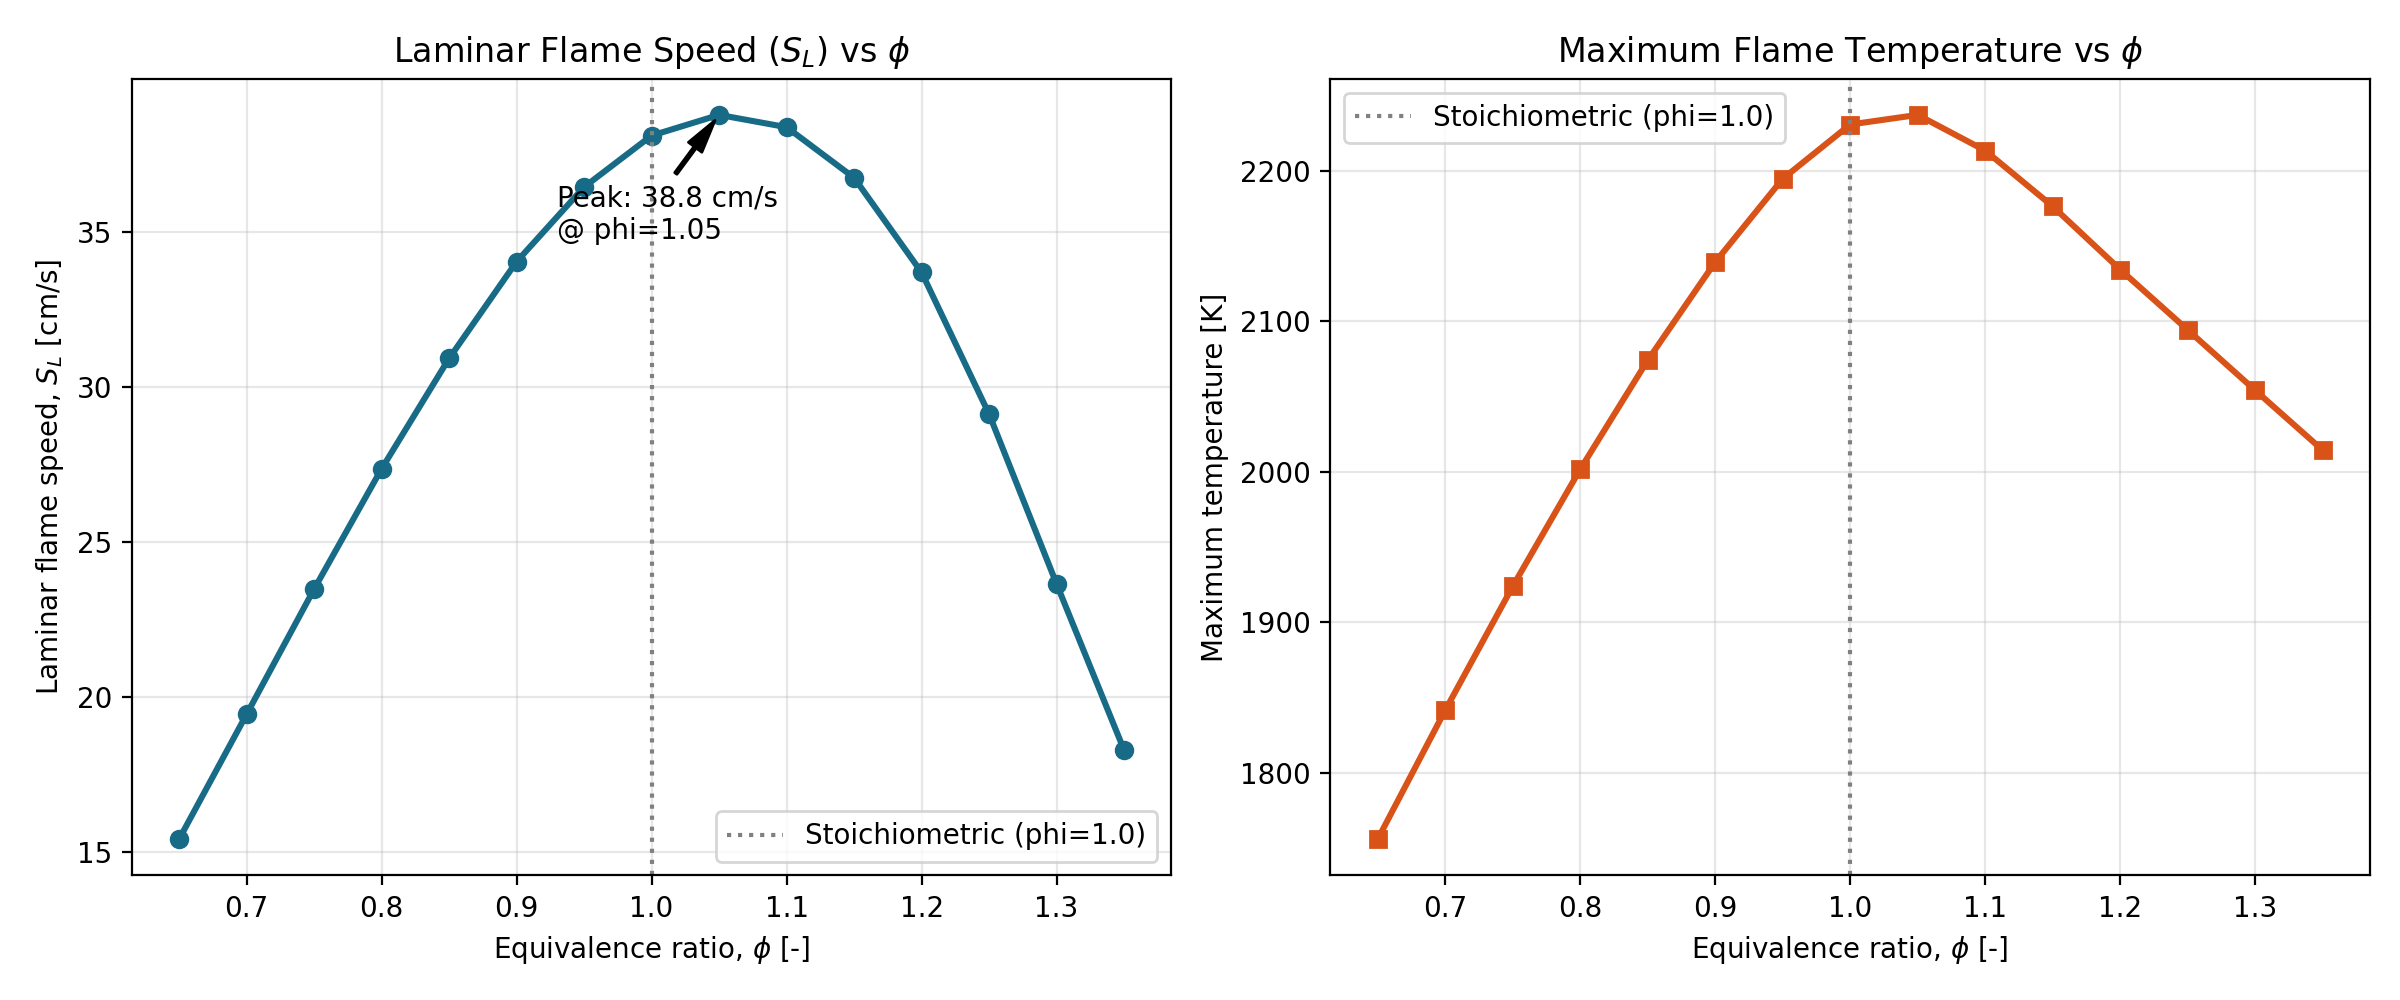
\includegraphics[width=\textwidth]{flame_results/graphs/01_summary_vs_phi.png}
  \end{column}

  \begin{column}{0.46\textwidth}
    \small
    \begin{tabular}{cccc}
      \toprule
      $\phi$ & Regime & $S_L$ [cm/s] & $T_{\max}$ [K] \\
      \midrule
      0.70 & Lean & 19.44 & 1841.4 \\
      0.80 & Lean & 27.35 & 2001.6 \\
      0.90 & Lean & 34.03 & 2139.3 \\
      \textbf{1.00} & \textbf{Stoich.} & \textbf{38.09} & \textbf{2230.7} \\
      \textbf{1.10} & \textbf{Rich} & \textbf{38.36} & 2213.4 \\
      1.20 & Rich & 33.68 & 2134.3 \\
      1.30 & Rich & 23.64 & 2054.1 \\
      \bottomrule
    \end{tabular}
    \vspace{0.5em}
    \begin{itemize}
      \item $T_{\max}$ peaks at $\phi = 1.00$ ($2230.7\text{ K}$).
      \item $S_L$ peaks at $\phi = 1.10$ ($38.36\text{ cm/s}$) due to maximal radical production ($H, OH$).
    \end{itemize}
  \end{column}
\end{columns}
\end{frame}

% -----------------------------------------------------------------------------
% Slide 5: Results — Flame Physical Overview
% -----------------------------------------------------------------------------
\begin{frame}{Results: Flame Structure Overview ($\phi = 1.00$)}
\begin{columns}[c]
  \begin{column}{0.55\textwidth}
    \centering
    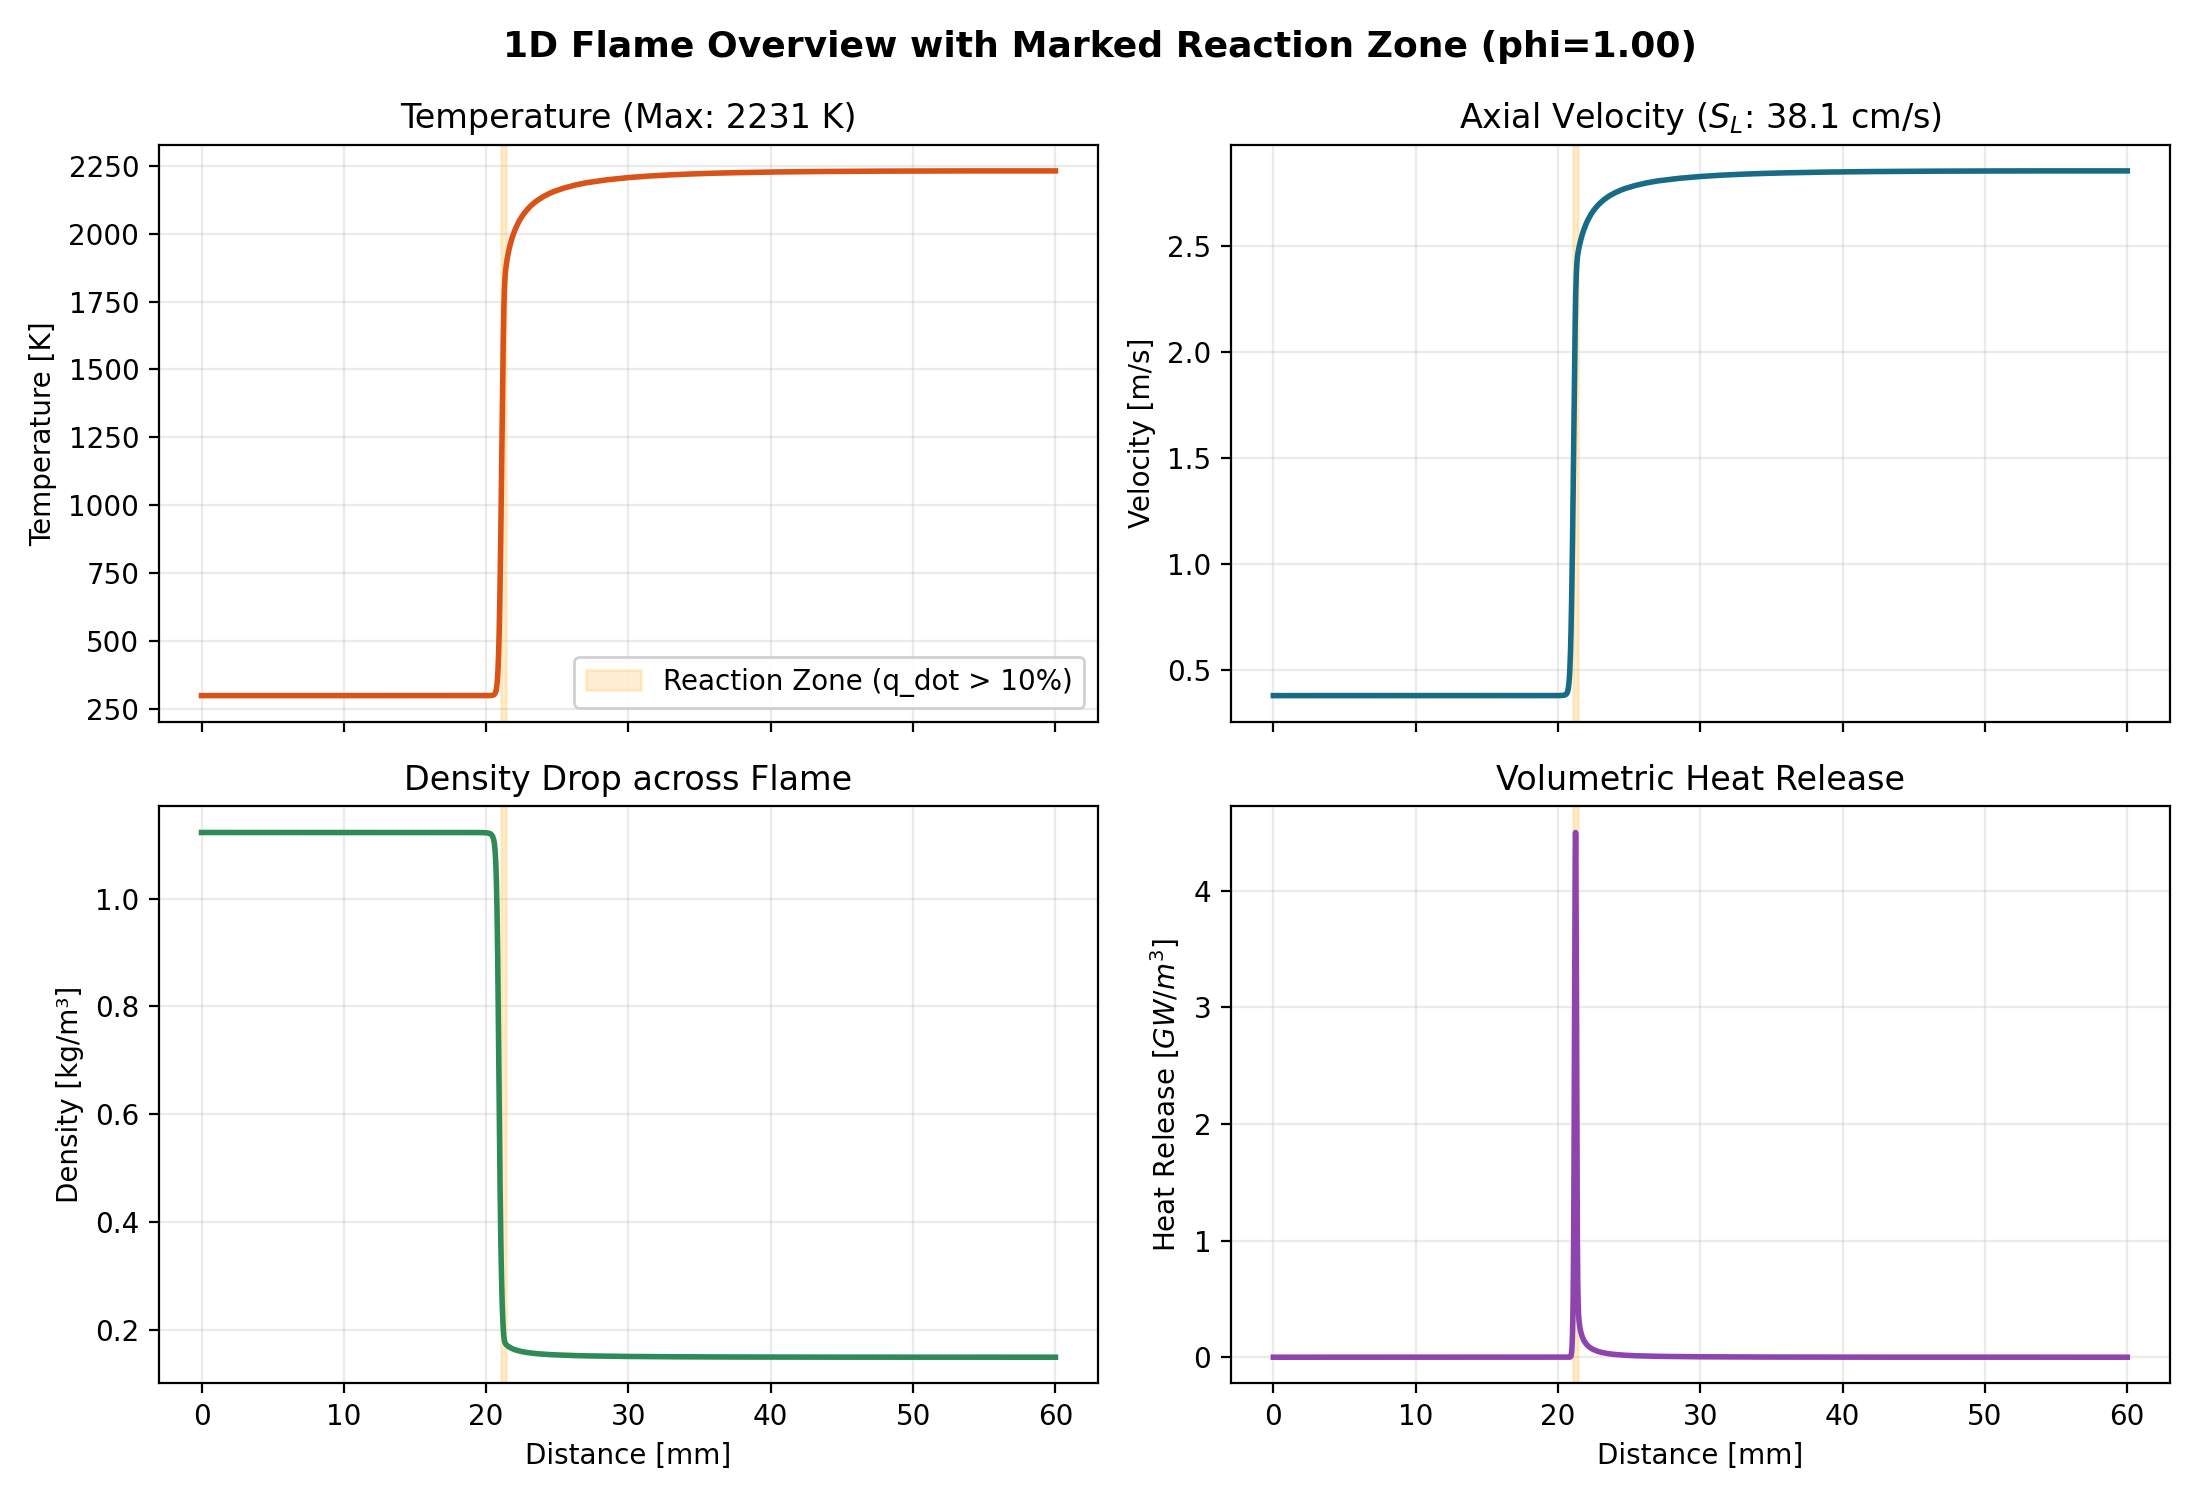
\includegraphics[width=\textwidth]{flame_results/graphs/02_physical_overview.png}
  \end{column}

  \begin{column}{0.43\textwidth}
    \textbf{Flame Zones Identified:}
    \begin{itemize}
      \item \textbf{Preheat Zone ($x < 21.06\text{ mm}$):} Conductive heat transfer preheats mixture from $300\text{ K}$ to $\sim 1300\text{ K}$.
      \item \textbf{Reaction Zone ($21.06 \le x \le 21.41\text{ mm}$):}
        \begin{itemize}
          \item Chemical reaction thickness: $\delta_{rxn} \approx 352\ \mu\text{m}$.
          \item Peak heat release: $4.50\text{ GW/m}^3$.
        \end{itemize}
      \item \textbf{Burned Zone ($x > 21.41\text{ mm}$):} Thermal expansion accelerates gas from $0.38\text{ m/s}$ to $2.87\text{ m/s}$ ($\rho u = \text{const}$).
    \end{itemize}
  \end{column}
\end{columns}
\end{frame}

% -----------------------------------------------------------------------------
% Slide 6: Results — Major Species & Radical Profiles
% -----------------------------------------------------------------------------
\begin{frame}{Results: Major Species \& Radical Pool}
\begin{columns}[c]
  \begin{column}{0.5\textwidth}
    \centering
    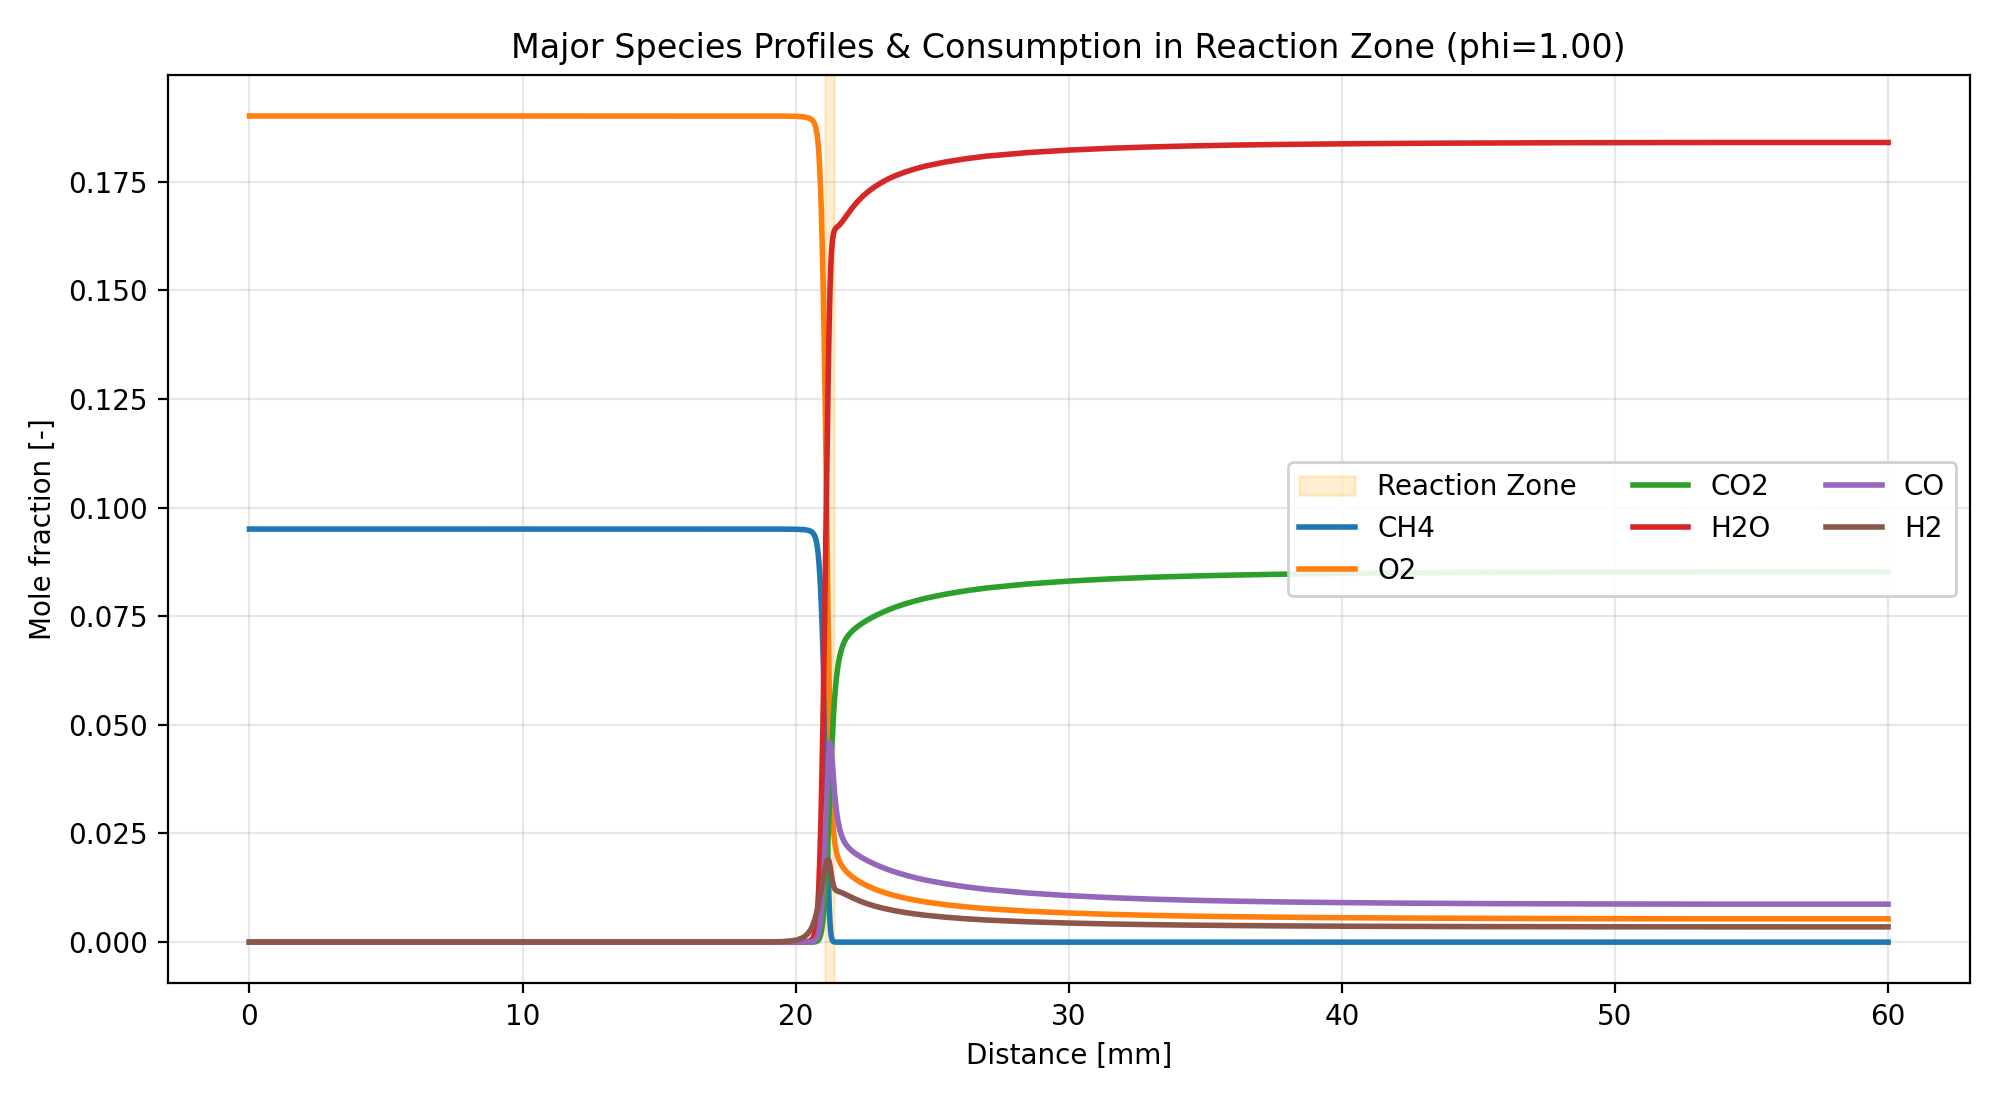
\includegraphics[width=\textwidth]{flame_results/graphs/03_major_species.png}
    \vspace{-0.5em}
    \captionof*{figure}{\footnotesize Major Species ($CH_4, O_2, CO, CO_2, H_2O$)}
  \end{column}

  \begin{column}{0.5\textwidth}
    \centering
    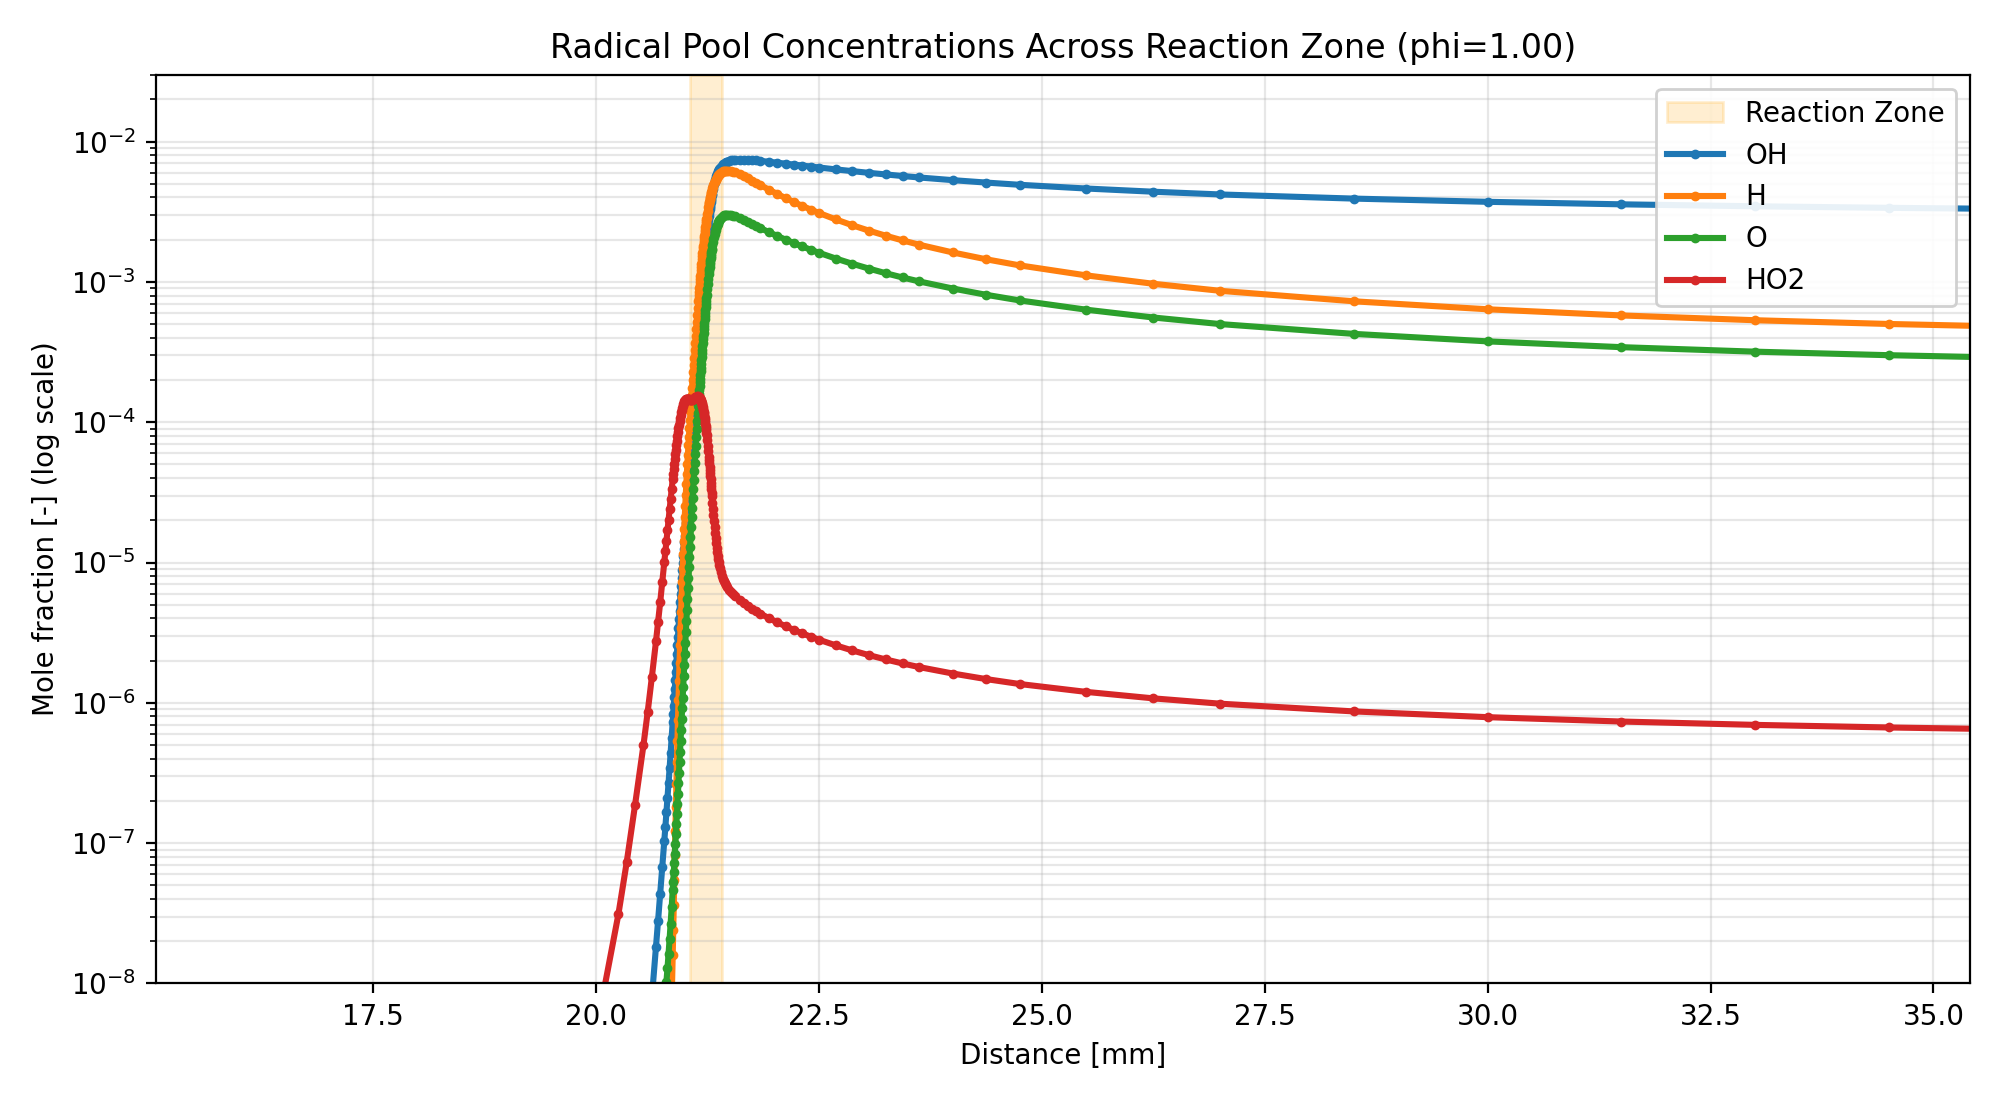
\includegraphics[width=\textwidth]{flame_results/graphs/04_radicals_log_scale.png}
    \vspace{-0.5em}
    \captionof*{figure}{\footnotesize Radicals on Log Scale ($OH, H, O, HO_2$)}
  \end{column}
\end{columns}
\vspace{0.3em}
\footnotesize
\textbf{Insight:} Radicals peak sharply within the $350\ \mu\text{m}$ reaction zone ($X_k \sim 10^{-3}$ to $10^{-6}$), sustaining high-temperature chain-branching.
\end{frame}

% -----------------------------------------------------------------------------
% Slide 7: Results — Key Chemical Reactions
% -----------------------------------------------------------------------------
\begin{frame}{Chemical Kinetics Diagnostics}
\begin{columns}[c]
  \begin{column}{0.55\textwidth}
    \centering
    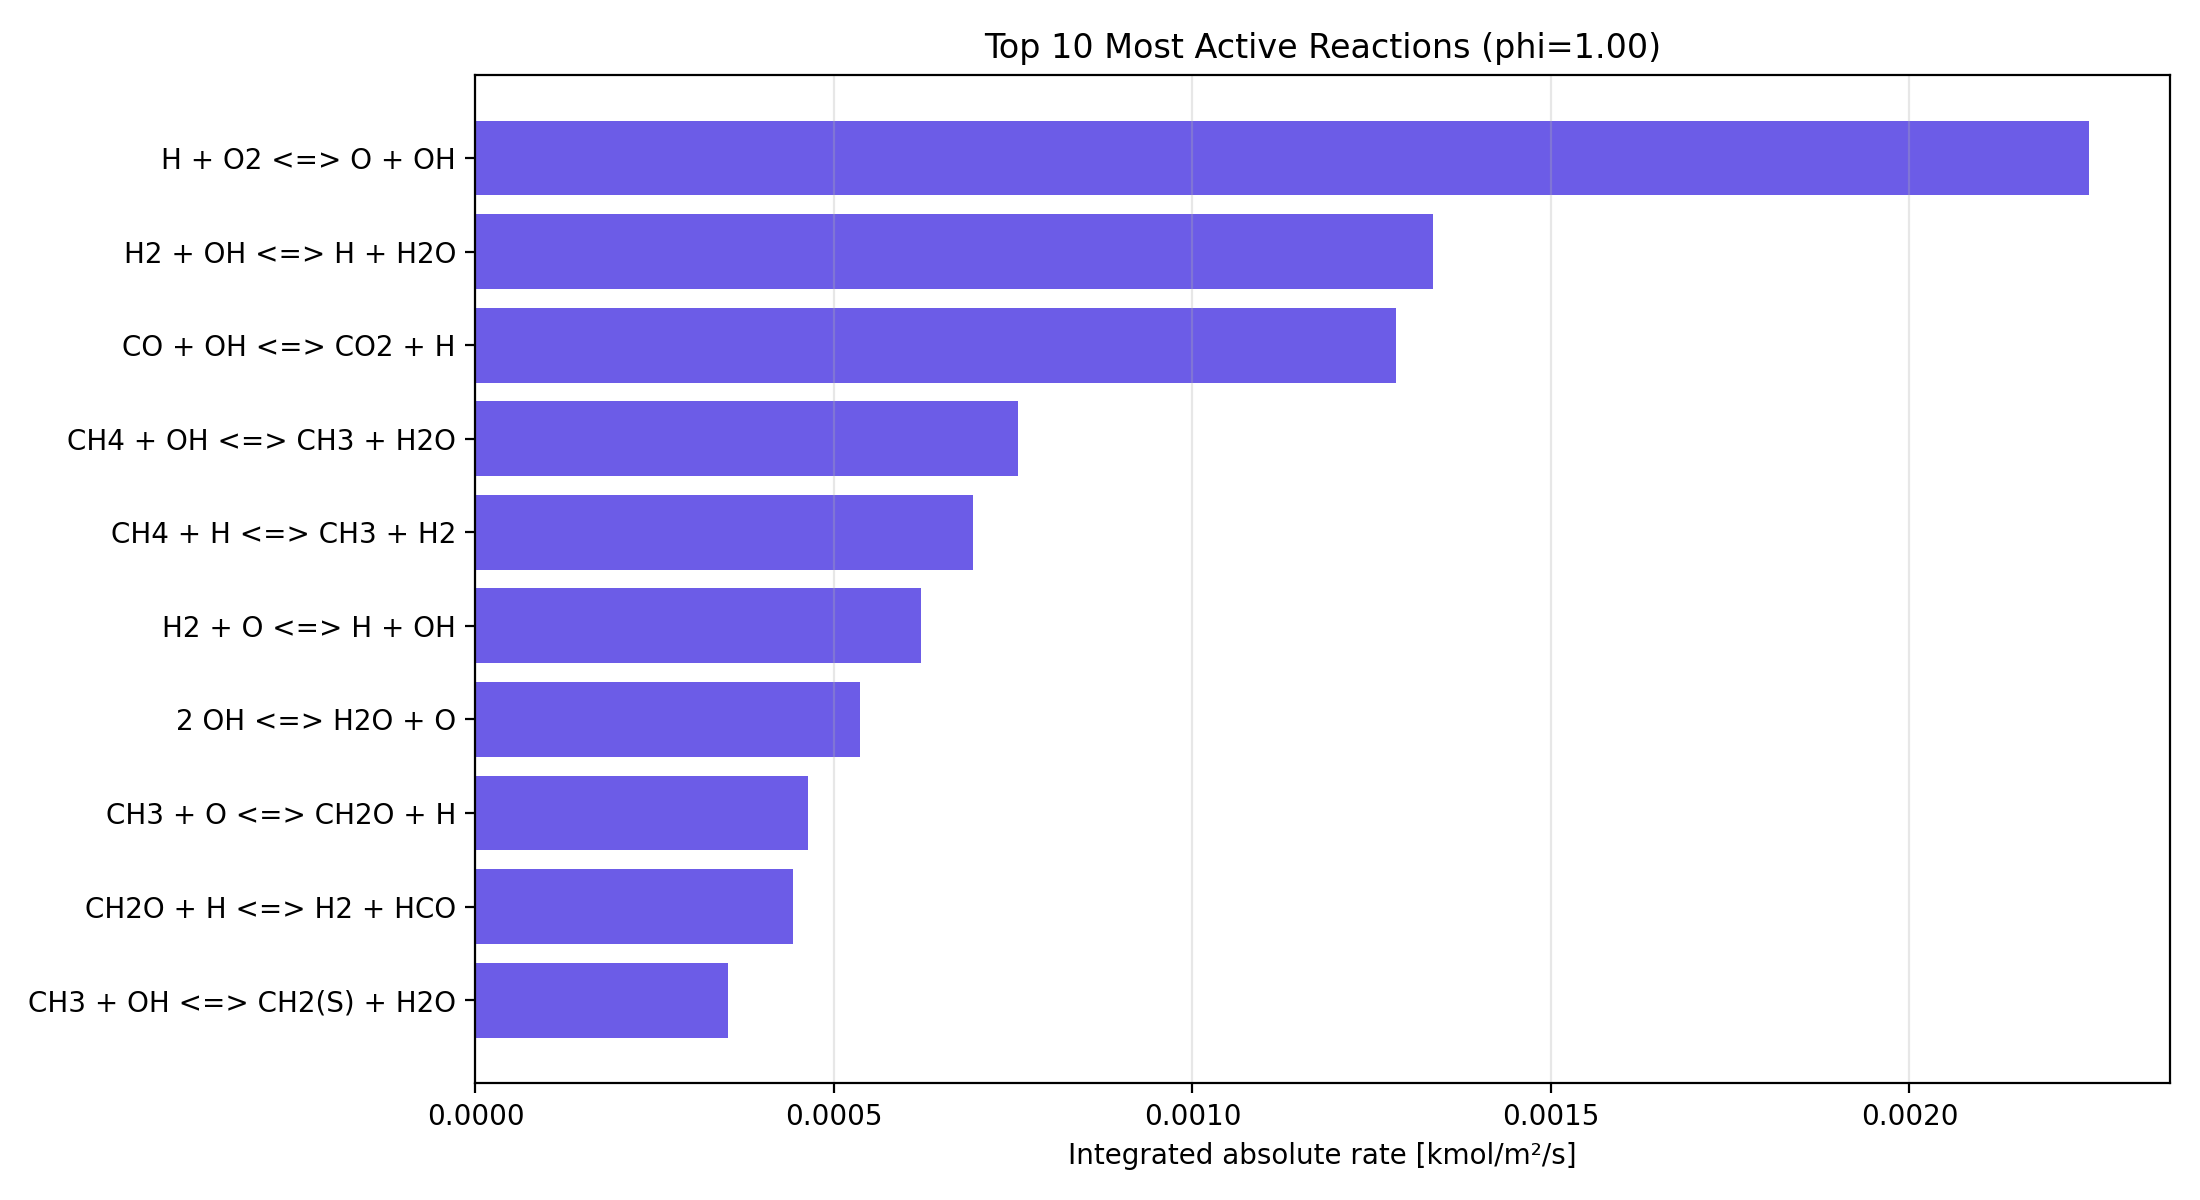
\includegraphics[width=\textwidth]{flame_results/graphs/06_top_reactions.png}
  \end{column}

  \begin{column}{0.43\textwidth}
    \textbf{Top Integrated Reactions:}
    \begin{enumerate}
      \item \textbf{Primary Chain Branching:}
        $$\text{H} + \text{O}_2 \rightleftharpoons \text{O} + \text{OH}$$
        \textit{Controls overall flame speed.}
      \item \textbf{Exothermic Heat Release:}
        $$\text{CO} + \text{OH} \rightleftharpoons \text{CO}_2 + \text{H}$$
        \textit{Drives temperature rise.}
      \item \textbf{Radical Chain Propagation:}
        $$\text{OH} + \text{H}_2 \rightleftharpoons \text{H}_2\text{O} + \text{H}$$
    \end{enumerate}
  \end{column}
\end{columns}
\end{frame}

% -----------------------------------------------------------------------------
% Slide 8: Multi-Equivalence Ratio Comparison
% -----------------------------------------------------------------------------
\begin{frame}{Multi-$\phi$ Comparison \& Reaction Layer Diagnostics}
\begin{columns}[c]
  \begin{column}{0.52\textwidth}
    \centering
    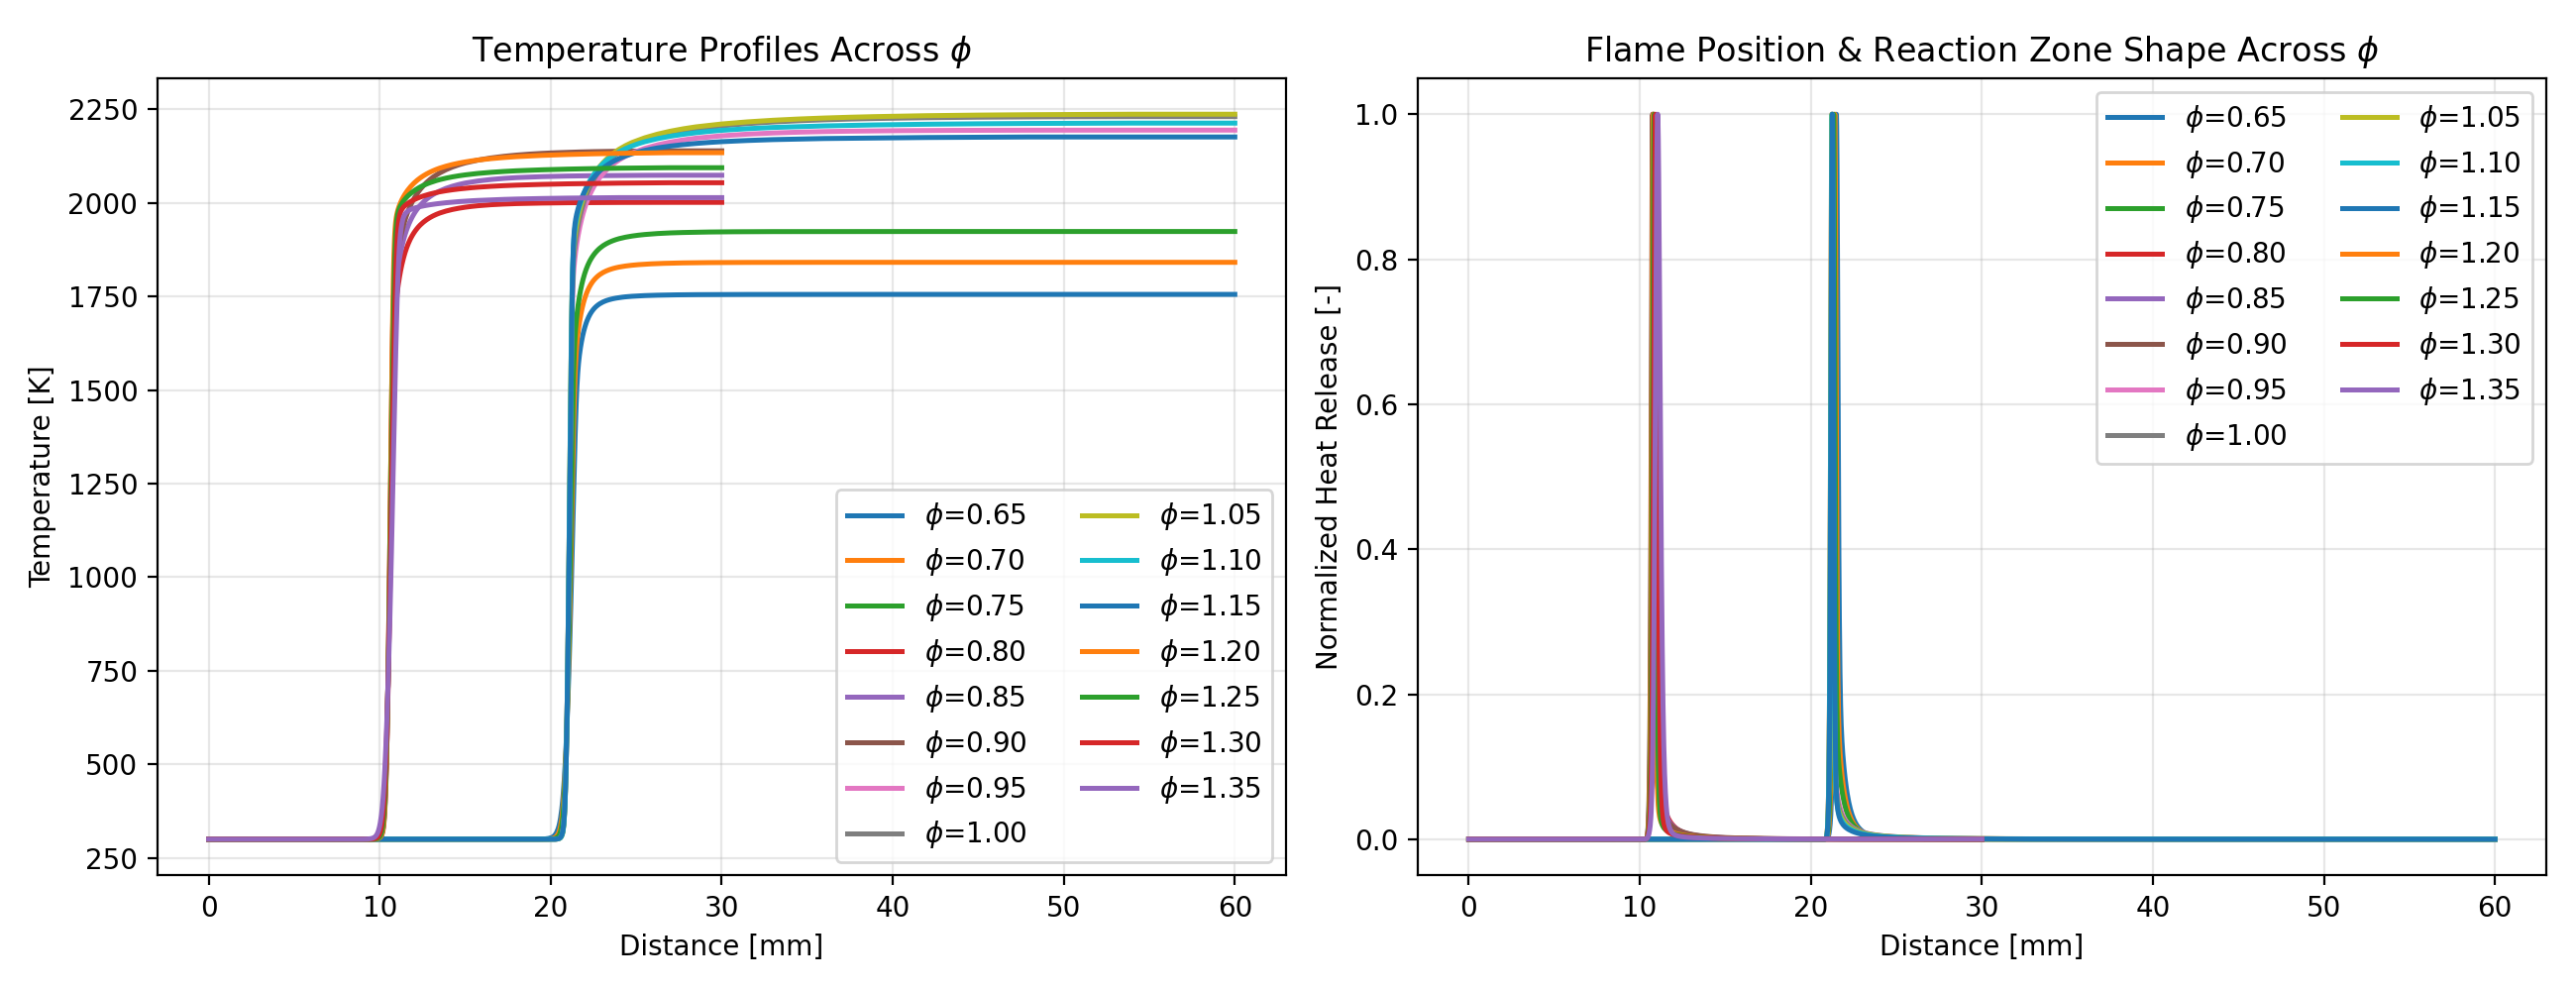
\includegraphics[width=\textwidth]{flame_results/graphs/08_multi_phi_profiles.png}
  \end{column}

  \begin{column}{0.46\textwidth}
    \textbf{Structure Across Equivalence Ratios:}
    \begin{itemize}
      \item Near stoichiometric ($\phi = 1.0 - 1.1$), flame temperature gradients are steepest, yielding the thinnest reaction zones ($\delta_T \approx 0.43\text{ mm}$).
      \item Lean ($\phi=0.7$) and rich ($\phi=1.3$) flames exhibit broader reaction zones ($\delta_T \approx 0.62 - 0.66\text{ mm}$).
      \item Direct physical correlation:
        $$\text{Thinner Reaction Zone} \longleftrightarrow \text{Higher } S_L$$
    \end{itemize}
  \end{column}
\end{columns}
\end{frame}

% -----------------------------------------------------------------------------
% Slide 9: Model Validation against Standards
% -----------------------------------------------------------------------------
\begin{frame}{Numerical Verification \& Literature Validation}
\begin{block}{1. Laminar Flame Speed ($S_L$ at $\phi = 1.0$, $1\text{ atm}$, $300\text{ K}$)}
\begin{itemize}
  \item Standard GRI-Mech 3.0 literature benchmark: $38.0 - 39.0\text{ cm/s}$
  \item \textbf{Our Model:} \textbf{$38.09\text{ cm/s}$} ($\Delta < 0.2\%$)
\end{itemize}
\end{block}

\begin{block}{2. Adiabatic Flame Temperature ($T_{ad}$)}
\begin{itemize}
  \item Equilibrium Literature: $\approx 2225 - 2235\text{ K}$
  \item \textbf{Our Model:} \textbf{$2230.7\text{ K}$} (Full thermodynamic agreement)
\end{itemize}
\end{block}

\begin{block}{3. Mass Flux Conservation ($\rho \cdot u$)}
$$\rho_u u_u = 1.130 \times 0.3809 = 0.430\text{ kg/(m}^2\cdot\text{s})$$
$$\rho_b u_b = 0.150 \times 2.8710 = 0.430\text{ kg/(m}^2\cdot\text{s}) \quad (\text{Error} = 0.00\%)$$
\end{block}
\end{frame}

% -----------------------------------------------------------------------------
% Slide 10: Conclusions
% -----------------------------------------------------------------------------
\begin{frame}{Conclusions}
\begin{enumerate}
  \item \textbf{Comprehensive 1D Flame Modeling:} Successfully simulated freely-propagating methane-air flames across $\phi = 0.70 - 1.30$ using GRI-Mech 3.0 detailed kinetics.
  \item \textbf{Peak Phenomena Verified:} Maximum temperature occurs at $\phi = 1.00$ ($2230.7\text{ K}$), whereas maximum flame speed peaks at $\phi = 1.10$ ($38.36\text{ cm/s}$) due to radical enhancement.
  \item \textbf{Spatial Layering Quantified:} Reaction zone is sub-millimeter thin ($\approx 352\ \mu\text{m}$), preceded by a conductive preheat zone.
  \item \textbf{Validation:} Numerical outputs show exact agreement with standard combustion literature.
\end{enumerate}

\vspace{1em}
\centering
\textbf{Thank you! Questions \& Discussion.}
\end{frame}

\end{document}
